% ESTE ES EL PAPER ESTUDIANDO LOS DOMINIOS DEL MAPA DE SPROTT EN PUNTO FIJO
% la idea es hacer una version de este paper para mandar a Chaos, Solitons and Fractals FI 1.222.
% otra posibilidad es mandarlo a Communications in Nonlinear Science and Numerical Simulation, Elsevier Science, ISSN 1007-5704, FI 2.88
\documentclass{elsart}
%%%%%%%%%%%%%%%% The amssymb package provides various useful mathematical symbols
\usepackage{amssymb}
%%%%%% Para los graficos:
\usepackage[pctex32]{graphics}
\usepackage{graphicx}
\graphicspath{{converted_graphics/}}
% la idea es hacer una version de este paper para mandar a Chaos, Solitons and Fractals FI 1.222.
% otra posibilidad es mandarlo a Communications in Nonlinear Science and Numerical Simulation, Elsevier Science, ISSN 1007-5704, FI 2.88

\begin{document}

\newcommand{\be}{\begin{equation}}
\newcommand{\ee}{\end{equation}}
\newcommand{\ben}{\begin{eqnarray}}
\newcommand{\een}{\end{eqnarray}}
\newcommand{\nn}{\nonumber \\}
\newcommand{\ii}{\'{\i}}
\newcommand{\pp}{\prime}
\newcommand{\nd}{{\noindent}}

\begin{frontmatter}

% paper title
\title{Nontrivial behavior of the fixed-point version of $2D$-chaotic maps}
\author[mdp,CONICET]{Luciana De Micco},
\ead{lucianadm55@gmail.com}
\author[mdp]{Maximiliano Antonelli},
\ead{maxanto@gmail.com}
\author[mdp,CONICET]{Hilda A. Larrondo}
\ead{larrondo@fi.mdp.edu.ar}

\address[mdp]{Departamentos de F\'{i}sica y de Ingenier\'{i}a Electr\'{o}nica,\\
              Facultad de Ingenier\'{\i}a,Universidad Nacional de Mar del Plata.\\
              Av. Juan B. Justo 4302, 7600 Mar del Plata, Argentina}
\address[CONICET]{Fellow of CONICET-Argentina}

\begin{abstract}
This paper deals with a family of interesting $2D$-quadratic maps first proposed by Sprott, in his seminal paper \ref{Sprott1993}, to generate chaotic ''art". Our main interest in these maps is they may be used to generate a novel encryption system, because they present multiple chaotic attractors depending on the selected point in the parameter's space.  Only the continuous case of these maps has been published in the open literature. The objective of this paper is to extend the study to the digital version, to make possible  the hardware implementation in fixed point arithmetics. Our main contributions are: (a)  the determination of a threshold of the bus width required in order to preserve the domain of attraction of the chaotic attractor and (b) the use of three quantifiers to confirm that this minimal bus width is enough to preserve main statistical characteristics of the continuous system. The quantifiers are the Maximum Lyapunov Exponent ($MLE$) and the Normalized Shannon Entropy ($H$), applied to two different Probability Density Functions (PDFs).
PACS:xxxx
\end{abstract}

\maketitle
\end{frontmatter}
{\bf VERSION: \today}

\section{Introduction} \label{sec:intro}
% ==================================================
% resumen
%% LO QUE VAMOS A CONTAR EN ESTE PAPER ES LO SIGUIENTE:
%primero mostramos algunos atractores en flotante
%para uno de esos a tractores mostramos los dominios de atracci�n
%
%segundo contamos como estudiamos la degradaci�n de los dominios de atracci�n.
%tercero contamos como estudiamos la degradaci�n de las variables de estado del sistema, es decir de la serie temporal generada por el sistema
%cuarto contamos como implementamos
%mostramos los resultados concretos obtenidos para la degradaci�n de los dominios de atracci�n y para la degradaci�n de las variables de estado
% ==================================================
%
Digital hardware implementation of dynamical systems, requires the use of
a finite number of bits to represent the state variables. In spite only rational numbers may be represented in either a computer or a programable logic device, floating point architecture allows one to \textsl{recreate} the ideal continuous system's trajectories .

However, from an engineering point of view fixed point arithmetic is more efficient than floating point because it uses less resources and each operation requires a lower number of clock cycles. As a consequence power consumption is also diminished using fixed point arithmetics.

Chaotic systems has an increasing number of applications and their implementation is specially involved due to the \textsl{extreme sensitivity to initial conditions}. Among many chaotic systems available in the literature in this paper we are interested in a family of $2D$-maps \cite{Sprott1993} proposed by Sprott,  and modeled by a pair of coupled quadratic equations:

\begin{eqnarray}\label{eq:mapaSprott}
x_{n+1}=a_1~+~a_2~ x_n~+~a_3 ~x_n^2~+~a_4 ~x_n~ y_n~+~a_5 ~y_n~+~a_6~ y_n^2\\
y_{n+1}=a_7~+~a_8~ x_n~+~a_9 ~x_n^2~+~a_10 ~x_n~ y_n~+~a_11 ~y_n~+~a_12~ y_n^2
\end{eqnarray}

where $\{x,y\}$ are the state variables and $\{a_i, i=1,...,12\}$ are the parameters. Using floating point arithmetics Sprott shaw that by automatic swept of parameters $a_i$ a hugh number of points in the parameter's space (about $6~10^{16}$) having a chaotic permanent regime may be detected. Furthermore Sprott found a correlation between the correlation dimension and the Lyapunov exponents of these chaotic attractors with their  \textsl{visual appeal}, an issue with interest for automatic \textsl{art} generation.

Let us consider here the digital version of this family of $2D$-maps. Several strategies has been proposed for a correct selection of the optimal number of
bits in hardware implementations. However, most of the methods proposed
in the literature are limited to linear systems
\cite{Constantinides2002,Constantinides2003}. But in digital chaotic systems a completely
different behavior may be obtained by varying the precision.  This issue  has
gained interest recently and several new schemes have been proposed
\cite{Ding2007,Aseeri2002,Azzaz2009}.

Grebogi's work \cite{Grebogi1988} showed that the average
length of periodic orbits (T) of a dynamical system implemented in a computer scales as a
function of the computer precision (e) and the correlation dimension
 of the chaotic attractor: $T \sim  e^{-d/2}$. In
\cite{SHUJUN2005} some findings on a new series of dynamical
indicators, which can quantitatively reflect the degradation
effects on a digital chaotic map realized with a fixed-point
finite precision have been reported. They are restricted to $1D$
piecewise linear chaotic maps (PWLCM). 

In this work we developed a detailed analysis of the \textsl{degradations} of the multiatractor chaotic system modeled by Eq. \ref{eq:Sprott} a fixed point implementation. By \textsl{degradation} we mean:  (a) the appearance of stable iced points and stable periodic orbits with short periods, inside a floating point domain of attraction without stable orbits; (b) the attractor itself becomes periodic and its statistical characteristics change, making the system more deterministic.
The main contributions are: (a) the analysis of the domains of attraction of the chaotic attractors for a given set of parameters as the number of bits encoding the decimal part of the number increases; the appearance of stable fixed points and periodic orbits with short periods is analyzed. (b) the determination of a threshold width for the
bus in order to keep the same statistical desired properties in the digital system as the continuous system has. We use two quantifiers to evaluate the statistical properties of the implementation using a different bus width: a) the Maximum Lyapunov Exponent (MLE) that measures sensitivity to initial condition with a positive value for chaotic behavior b)  the Normalized Shannon Entropy (H), using two different PDF's: one of them is the normalized histogram of the time series; the other is the histogram of ordering patterns of the time series. These quantifiers have abrupt changes at specific bus widths.

The work is organized as follows: section \ref{sec:caos} gives a brief description of the
chaotic system analyzed. In section \ref{sec:degattract} a detailed explanation of how the
digitalization is performed and the analysis of the degradations of the domains of attraction is
performed. Section \ref{sec:repre} describes the quantifiers and the method to quantify the degradation of the attractor itself. We give experimental result in Section \ref{sec:results}.
Finally, the conclusions and future work are given in section
\ref{sec:conclusions}.
%========================================================================================
\section{Caotic system under study}
\label{sec:caos}

The  family of $2D$ quadratic maps studied is given by \ref{eq:mapaSprott} above.The $12$
coefficients $a_i$ define a $12D$ parameters space that is very hard to be explored.
Sprott discovered that this set of equations produce a huge number of chaotic attractors (about $6~10^{16}$) in floating point arithmetics. Three of them are shown in Fig. \ref{fig:atractores}
\begin{figure}
    \centering
    \includegraphics[width=1\columnwidth]{atractoreslindos}\\
    \caption{Three attractors for three different sets of  coefficients $a_i=\{-1.0,~0.9,~0.4,~-0.2,~ -0.6,~
-0.5, ~0.4, ~0.7, ~0.3, ~-0.5, ~0.7, ~-0.8\}$ .}\label{fig:atractores}
\end{figure}

ATENCION LUCIANA LA FIGURA TIENE 3 ATRACTORES Y HAY UN SOLO JUEGO DE PARAMETROS.



Fig. \ref{fig:atrac} shows the floating point domain of attraction of Eq. \ref{eq:mapaSprott}  for
parameters $a_i=\{-1,0.9,0.4,-0.2,-0.6,-0.5,0.4,0.7,0.3,-0.5,0.7,-0.8\}$. In this Fig. each pair $[x,y]$ is an initial
condition. The color assigned to each pair depends on the permanent regime reached by the system, starting from that particular point. Grey colored points constitute the domain of attraction of the chaotic attractor overimposed in black.

\begin{figure}
    \centering
    \includegraphics[width=1.1\columnwidth]{atractorcondimension1}\\
    \caption{Domain of attraction (in grey) and chaotic attractor (in black) of the system of Eq. \ref{eq:mapaSprott} in floating point arithmetics. Parameters values are: $a_i=\{-1.0,~0.9,~0.4,~-0.2,~ -0.6,~
-0.5, ~0.4, ~0.7, ~0.3, ~-0.5, ~0.7, ~-0.8\}$ }\label{fig:atrac}
\end{figure}
%========================================================================================
\section{Degradation of the domains of attraction}
\label{sec:degattract}

Inside the floating point attractor's domain a number of initial conditions not converging to the attractor appear in fixed point arithmetics. Some of these points diverge to infinity. Other point become stable fixed points or low period stable periodic orbits.

The maximum theoretical period that can be reached in a system with $d$ dimensional state space, using $n_b$ bits to represent the state variables is: $2^{d*n_b}$. For example for $d=2$ and $n_b=10$ the maximum theoretical period for the system in Eq. \ref{eq:mapaSprott} is $2^{(2*10)} = 1048576$. But actually stable periodic orbits with lower periods appear, depending on the initial conditions. This low period stable orbits do not exist in floating point arithmetics. As a consequence if one wants to obtain a similar behavior in fixed point arithmetics the \textsl{degradation} of the domain of attraction is one measure of the  \textsl{degradation} of the hardware implementation using a bus with the same number of bits than the fixed point representation of the state variables.

We  systematically studied the behavior of the system starting from a grid of initial conditions inside the floating point domain of attraction,
using different precisions, in a fixed point architecture,
that emulatese a FPGA implementation. Our interest is to measure how the attraction domain
degrades with the variation of the bits employed, as well as to find a threshold value for $n_b$ above which the chaotic
behavior of the system appears.
=======================================================
%+++++++++++++++++++++++++++++++++
EL PARRAFO QUE SIGUE LO SACO PORQUE NO AGREGA NADA NUEVO
%If you choose initial values of X and Y somewhere near the
%attractor, within its basin of attraction, and substitute these
%values into the equations that describe the attractor, the new
%values of X and Y represent a point in the plane that is closer to
%the attractor. After a number of iterations, the point works its
%way to the attractor, and thereafter it moves around on the
%attractor in some complicated manner, eventually visiting every
%part of the attractor. The next position can always be simply and
%accurately predicted from the current position, but the small,
%inevitable uncertainty in position continually increases so that a
%long term prediction is impossible, except to say that the point
%is somewhere on the attractor. You can think of the attractor as
%the set of all possible long-term solutions of the equations that
%produced it.
%

%Besides the error in knowing perfectly the initial conditions,
%there are also computer round-off errors at each iteration. Given
%the extreme sensitivity to small errors, you may wonder whether
%any computer is capable of calculating correctly such a chaotic
%process. It is true that if the same chaotic equations are
%iterated on two computers using different precision or round-off
%methods, the sequence of iterates is almost certainly completely
%different after a few dozen iterations. However, the appearance of
%the attractor is probably the same. In such a case, we say that
%the solution is structurally stable or robust. Furthermore,
%according to the shadowing lemma, an appropriate small change in
%initial conditions produces a chaotic sequence that follows
%arbitrarily close to the computed one.
%
=======================================================
%Since computers always round the results of calculations to a
%finite number of digits (or more precisely, bits), a limited
%number of values is allowed. Thus successive iteration of a map
%always eventually repeats a previously obtained value, whereupon
%the solution reproduces exactly the same sequence of states as it
%did before. Strictly speaking, every such solution is periodic,
%and true chaos cannot be observed with a computer. However, with
%double-precision floating point variables, which are normally 64
%bits, there are 264 or about 1019 possible values. It can be shown
%that an average periodicity occurs after about the square root of
%this number of iterations, which is about 3 x 109. Until the
%number of iterations approaches this value, there is little cause
%to worry. For maps higher than one dimension, this problem is even
%less serious because all the variables have to reach a previously
%existing state at the same time.



 CORREGIR PRIMERO HASTA ACA
\section{Degradations of the state variables' time series}
\label{sec:degstatevar}
From a statistic point of view two main characteristics of a digital dynamical system must be measure: *(a) the distribution of the values of its state variables over all the possible values and (b) the independence between consecutive values. For example a pseudo random number generator must have a uniform distribution and consecutive values must be independent from each other. 

In previous works devoted to \emph{PRNG}'s, the use of two Probability Distribution Functions (\emph{PDF}'s has been useful for comparison between different systems. One \emph{PDF}  is the normalized histogram and the quantifier is the normalized Shannon entropy of this \emph{PDF}. The other one is the \emph{PDF} proposed by Bandt \& Pompe \cite{Pompe2002} and the quantifier is again its normalized Shannon entropy. Let us summarize how the second \emph{PDF} is obtained.

\subsubsection{PDF based on histograms}

In order to  extract a PDF via amplitude-statistics, divide first
the interval $[0,1]$ into a finite number $nbin$ of non
overlapping subintervals $A_i$: $[0,1]=\bigcup_{i=1}^{nbin} A_i$
and $A_i\bigcap A_j=\emptyset~\forall i\neq j$. One then employs
the usual histogram-method, based on counting the relative
frequencies of the time series values within each subinterval. It
should be clear that the resulting  PDF lacks any information
regarding temporal evolution. The only pieces of information we
have here are the $x_i-$values that allow one to assign inclusion
within a given bin, ignoring just where they are located (this is,
the subindex $i$.)


\subsubsection{PDF based on Band and Pompe methodology}
%
Let $x$ be the state variable considered and let $x_1$ to $x_N$ be its digital time series.
To use the Bandt and Pompe \cite{Pompe2002} methodology for evaluating
of probability distribution $P$ associated to the time series
(dynamical system) under study one starts by  considering
partitions of the pertinent $D$-dimensional space that will
hopefully ``reveal" relevant details of the ordinal-structure of a
given one-dimensional time series $ \{x_t : t=1, \cdots,M \}$ with
 embedding dimension $D > 1$. We are interested in ``ordinal
patterns" of order $D$ \cite{Pompe,Keller} generated by
\begin{equation}
(s)~\mapsto~
\left(~x_{s-(D-1)},~x_{s-(D-2)},~\cdots,~x_{s-1},~x_{s}~\right) \,
 \label{eq:vectores}
\end{equation}
which assign to each time $s$ the $D$-dimensional vector of values
at times $s, s-1,\cdots,s-(D-1)$. Clearly, the greater the
$D-$value, the more information on the past  is incorporated into
our vectors. By the ``ordinal pattern" related to the time $(s)$
we mean the permutation $\pi=(r_0,r_1, \cdots,r_{D-1})$ of
$(0,1,\cdots,D-1)$ defined by
\begin{equation}
x_{s-r_{D-1}}~\le~x_{s-r_{D-2}}~\le~\cdots~\le~x_{s-r_{1}}~\le~x_{s-r_0}
\ . \label{eq:permuta}
\end{equation}
In order to get a unique result we set $r_i <r_{i-1}$ if
$x_{s-r_{i}}=x_{s-r_{i-1}}$. Thus, for all the $D!$ possible
permutations $\pi$ of order $D$, the probability distribution
$P=\{p(\pi)\}$ is defined by
\begin{equation}
p(\pi)~=~\frac{\sharp \{s|s\leq M-D+1;~ (s) \texttt{, has type
}\pi\}}{M-D+1} \ . \label{eq:frequ}
\end{equation}
In this expression, the symbol $\sharp$ stands for ``number".
================================================= llegue mas o menos hasta aca.

The Bandt-Pompe's methodology is not restricted to time series
representative of low dimensional dynamical systems but can be
applied to any type of time series (regular, chaotic, noisy, or
reality based), with a very weak stationary assumption (for $k =
D$, the probability for $x_t < x_{t+k}$ should not depend on $t$
\cite{Pompe}). One also assumes that enough data are available for
a correct attractor-reconstruction. Of course, the embedding
dimension $D$ plays an important role in the evaluation of the
appropriate probability distribution because $D$ determines the
number of accessible states $D!$. Also, it conditions the minimum
acceptable length $M \gg D!$ of the time series that one needs in
order to work with a reliable statistics.

\section{Maximum Lyapunov exponent}

The Lyapunov exponents are quantifiers that characterize how the
separation between two trajectories evolves, \cite{Sprott2003}. It
is generally well known that chaotic behaviors are characterized
mainly by Lyapunov numbers of the dynamic systems. If one or more
Lyapunov numbers are greater than zero, then the system behaves
chaotically, otherwise, the system is stable. In this paper, we
employ the maximum Lyapunov number as it is one of the most useful
indicators of chaos.

The distance between trajectories changes in $2^{MLE}$ for each
iteration, on average. If $MLE<0$ the trajectories approaches,
this may be due to a fixed point, if $MLE=0$ the trajectories keep
their distance, this may be due to a limit cycle, if $MLE>0$, the
distance between trajectories is growing, and is an indicator of
chaos. \cite{Sprott2003}

There is a non-analytical way to measure it if only the inputs and
outputs of the system are accessible. The procedure is the
following: The system must be started from two neighbor points in
the phase plane, lets call them $(x_a,y_a)$ and $(x_b,y_b)$, as
the system is iterated the Euclidean distance between the two
trajectories is measured ($d_n$ in the $n_{th}$ sample) (eq.
\ref{eq:D0D1}), and the b trajectory is relocalized on each
iteration  (eq. \ref{eq:reubicacion}), obtaining the points
$(x_{br},y_{br})$ to feed the system. Then the Lyapunov exponent
can be calculated as shown in eq. (\ref{eq:Lyapunov}). The process
can be seen in Fig. \ref{fig:relocalizacion}.


\begin{eqnarray}\label{eq:D0D1}
    d_{0(i-1)}&=& \sqrt{(x_{a(i-1)}-x_{br(i-1)})^2+(y_{a(i-1)}-y_{br(i-1)})^2}\nonumber\\
    d_{1(i)}&=& \sqrt{(x_{a(i)}-x_{b(i)})^2+(y_{a(i)}-y_{b(i)})^2}\\
\nonumber
\end{eqnarray}

\begin{eqnarray}\label{eq:Lyapunov}
    MLE &=& \frac{1}{M} \sum_{i=2}^{M} \log_2{\frac{d_{1(i)}}{d_{0(i-1)}}}
\end{eqnarray}


\begin{eqnarray}\label{eq:reubicacion}
    x_{br(i)}&=& x_{a(i)}+(x_{b(i)}-x_{a(i)})d_{o(i-1)}/d_{1(i)} \nonumber\\
    y_{br(i)}&=& y_{a(i)}+(y_{b(i)}-y_{a(i)})d_{o(i-1)}/d_{1(i)}
\end{eqnarray}


\section{ Digital Hardware Emulation.} \label{sec:repre}

A \textit{C} code that simulates the nonlinear system was developed and the quadratic map was reproduced as it would be
implemented in a digital hardware dispositive, for example a FPGA
implementation. The Code employs signed integer arithmetic and it
is equivalent to employ fixed point precision.


The system is intended to be working in decimal fixed point
architecture. It employs $4$ bits for representing the integer
part in $Ca_2$ convention ($m=4$) and it automatically scans the% que es $Ca_2$ convention???
number of bits to represent the fractional part of the number (n),
in order to analyze how the system reacts when the precision
changes.


For example in Table \ref{tab:tabla} there is the equivalence when% no entiendo que es lo que hay en la tabla???
using $n_{bits} =6$, $4$ bits for the integer part and $2$ bits
for the decimal part in $Ca_2$ convention ($m=4$ and  $n=2$).

\begin{table}[h]
  \caption{Table of equivalences.}\label{tab:tabla}
  \vspace{2mm}
  \centering
  \begin{tabular}{ c c c }
  Binary  & Decimal Fixed point & Signed Integer  \\
  $0111,11$ & $7,75$ & $31$ \\
  $0111,10$ & $7,5$ & $30$ \\
  $0111,01$ & $7,25$ & $29$ \\
   ... & ... &  ...\\
  $0000,00$ & $0$ & $0$  \\
  $1111,11$ & $-0,25$ & $-1$ \\
  $1111,10$ & $-0,5$ & $-2$  \\
   ... & ... & ... \\
    $1000,00$ &  $-8$ & $-32$  \\
  %  \hline
    \end{tabular}
\end{table}



Internally the FPGA works with binary numbers, designers must
interpret the bits based on the desired architecture. In order to
use the parameterizable operations provided by the FPGA's
libraries, that work with Signed Integer variables, an equivalence
between Decimal fixed point numbers and Signed Integers can be
done as shown in Table \ref{tab:tabla}.

The same binary number can be interpreted as an integer number or,
as in this case, if one wish to employ decimal numbers, interpret
a decimal point located at a desired position. This means:

\begin{equation}\label{eq:decimal}
number=-2^{(m-1)} ... 2^0,2^{-1}�2^{-n}
\end{equation}

where $n\_bits=m+n$.

In order to make this conversion, each decimal number must be
multiplied by $2^n$ to obtain the equivalent Signed Integer
number. Where $n$ is the quantity of bits used to represent the
decimal part of the number. This is equivalent to right-shift $n$
positions the decimal point.

\begin{equation}\label{eq:entero}
 number= -2^{(m-1+n)} ... 2^0
\end{equation}

where $n\_{bits}=m+n$.

The following considerations must be taken into account when operating with this equivalence:

\begin{itemize}
    \item Addition, this operation does not need any consideration just to make sure not to exceed the limits of the arithmetic used.
    \item Multiplication, the result of this operation must be divided by $2^n$ to adjust the result to the correct range.
    \item Division, the result must be always rounded towards minus infinity: $7.28$ to $7$ , $-14.9$ to $-15$.
\end{itemize}


The developed code iterates the Quadratic map white the following
coefficients:


$a_0=-1.0$, $a_1= 0.9$, $a_2= 0.4$, $a_3= -0.2$, $a_4= -0.6$,
$a_5= -0.5$, $a_6= 0.4$, $a_7= 0.7$, $a_8= 0.3$, $a_9=-0.5$,
$a_{10}= 0.7$ and $a_{11}= -0.8$.


Hence, the operations are done using signed integer variables that
are equivalent to decimal fixed point numbers, as it has been
explained in the previous section.

After each operation the corresponding adjustment is performed to work exactly as the FPGA does.


The map has been iterated with initial conditions $x_0$ and $y_0$
from  $-2$ to $2$ in steps of $0.001$, that means $16008001$
different points. On each case it was determined whether the
systems evolves to a fixed point, diverges or goes towards a
periodic cycle. It was also reported the repetition period of
these cycles.


For every value of precision $n$ we obtained a $4001$x$4001$ matrix whose elements correspond to each
initial condition. This means, the program outputs on each
position the final state of the system for that initial condition.

There are some desirable properties that constitutes a ``good"
PRNG, some of the most important ones are large period, few fixed
points and, of course, that do not diverge.

\section{Results} \label{sec:resultads}

Figures \ref{m5otro} to \ref{m16otro} display some of the results
(i.e. for some values of $n$) obtained, these are the set of final
states for each initial condition. With final state we mean: fixed
point, divergent point or the value of the period when the CI
converges to a cycle.

The abscissa and ordinate axis correspond to initial values of $x$
and $y$ respectively. They have been swept from $-2$ to $2$ in
steps of $0.001$.

It can be seen that for small values of $n$ the zone presents
bigger areas of divergent and fixed points. As the value of $n$
increases, it can be seen that the area of divergent points tends
to the one of the floating point (Fig. \ref{fig:atrac}).

Lower values of $n$ present irregular, or rough surfaces, with
predominant dark colors indicating that there is a prevalence of
 short periods cycles. As the value of $n$ increases the area smoothes and the
color tends to be lighter, indicating that the CIs converge to
higher periods cycles. This means that the range of initial values
that generate useful sequences increases for higher values of $n$.

\begin{figure}
    \centering
    \includegraphics[width=0.8\columnwidth]{Mapa2_m5}\\
    \caption{Domains of attraction $n=5$}\label{fig:m5otro}
\end{figure}

\begin{figure}
    \centering
    \includegraphics[width=0.8\columnwidth]{Mapa2_m6}\\
    \caption{Domains of attraction $n=6$}\label{fig:m6otro}
\end{figure}

\begin{figure}
    \centering
    \includegraphics[width=0.8\columnwidth]{Mapa2_m7}\\
    \caption{Domains of attraction $n=7$}\label{fig:m7otro}
\end{figure}

\begin{figure}
    \centering
    \includegraphics[width=0.8\columnwidth]{Mapa2_m10}\\
    \caption{Domains of attraction $n=10$}\label{fig:m10otro}
\end{figure}

\begin{figure}
    \centering
    \includegraphics[width=0.8\columnwidth]{Mapa2_m11}\\
    \caption{Domains of attraction $n=11$}\label{fig:m11otro}
\end{figure}



\begin{figure}
    \centering
    \includegraphics[width=0.8\columnwidth]{Mapa2_m14}\\
    \caption{Domains of attraction $n=14$}\label{fig:m14otro}
\end{figure}

\begin{figure}
    \centering
    \includegraphics[width=0.8\columnwidth]{Mapa2_m16}\\
    \caption{Domains of attraction $n=16$}\label{fig:m16otro}
\end{figure}

An analysis of these outputs can be seen in Figures
\ref{puntosfijos} to \ref{periodosmaximos}.

Fig. \ref{puntosdivergentes} and  \ref{puntosfijos} show the
quantity of points that diverge and converge to fixed points
respectively as the value of $n$ increases, in both cases the
final value tends to the floating point case. It is clear from
these figures that for $n \sim 12$ the system seems to behave
sufficiently accurate to the real one. However Figure
\ref{periodosmaximos} shows that a value of $12$ for $n$ the
system still have a quite short maximum period.


\begin{figure}
    \centering
    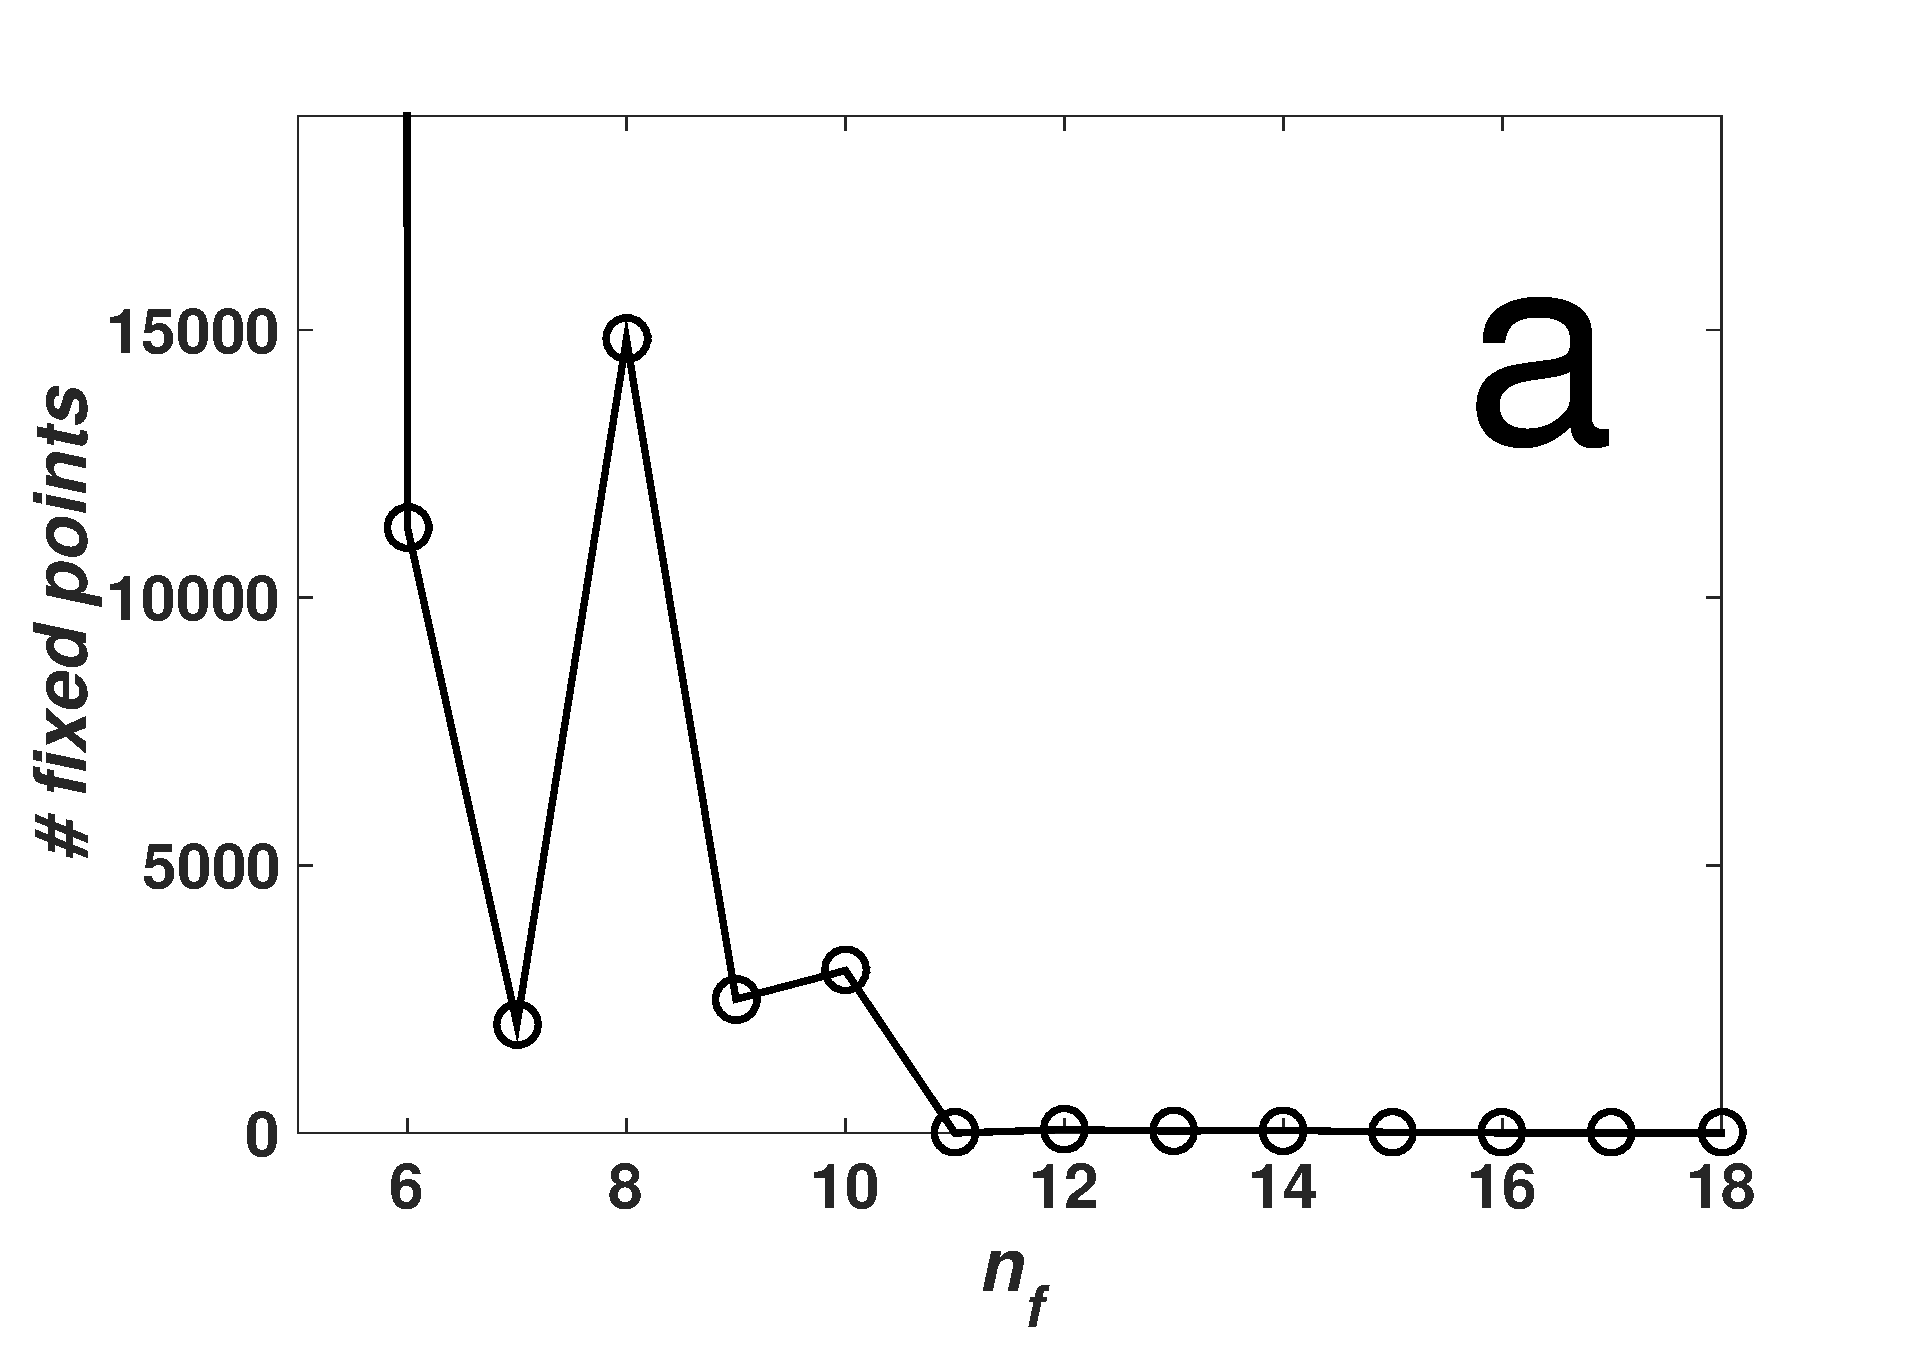
\includegraphics[width=0.7\columnwidth]{ptosfijos}\\
    \caption{Quantity of fixed points.}
    \label{fig:puntosfijos}

\end{figure}

\begin{figure}
    \centering
    \includegraphics[width=0.7\columnwidth]{divergen}\\
    \caption{Quantity of divergent points.}\label{fig:puntosdivergentes}

\end{figure}

\begin{figure}
    \centering
        \includegraphics[width=0.7\columnwidth]{periodosmaximos}\\
    \caption{Maximum periods reached.}\label{fig:periodosmaximos}

\end{figure}

\begin{figure}
    \centering
        \includegraphics[width=0.9\columnwidth]{Puntos}\\
    \caption{Quantity of initial conditions with period ($T$) higher and lower than $1000$.}\label{fig:puntos}

\end{figure}



\begin{figure}
    \centering
        \includegraphics[width=0.9\columnwidth]{HBP_Hhist}\\
    \caption{Quantifiers $H_{BP}$  and $H_{hist}$.}\label{fig:HBPHhist}

\end{figure}


Figure \ref{puntos} shows the quantity of initial conditions that
presents periods $T$ higher and lower than $1000$. Again, a value
of $12$ for $n$ seems to be the limit to obtain a good
approximation of system.

%
% this is
%interesting because in many applications these maps are intended
%to be used as controlled noise generators. So, to ensure long
%periods is required.
We realized that the analysis performed up to this point was not
enough to determine a conclusion, so we decided to further
analysis the data obtained by employing some statistical
quantifiers the Entropy applied to the $hist$ and $Band and Pompe$
distributions. Figure \ref{HBPHhist} shows the values of the
quantifier normalized Shannon entropy applied over two PDFs, the
histogram ($H_{hist}$) and Bandt-Pompe distribution ($H_{BP}$). In
the figure it can be seen that the two quantifiers tend to the
value calculated using floating-point arithmetic. While $H_{BP}$
is concordant with the previous analysis and shows that it
stabilizes for $n \sim 12$, $H_{hist}$ reaches the theoretical
value for $n \sim 19$, showing that there are properties of the
output sequences that only this quantifier can detect.

In Table \ref{MLE} the value of $MLE$ for some values of $n$. The
cases for $n=11, 12, 13$ and $25$ are showed. Also, the
theoretical value calculated with Matlab using floating point
arithmetic. It can be seen that as the value of $m$ increases the
$MLE$ tends to the theoretical value. Figure \ref{MLE} displays
 $MLE$ vs. $n$, there again the quantifier reaches the theoretical value at $n \sim 13$.

\centering

\begin{tabular}{|c|c|}

  \hline\label{tab:MLE}

  n & MLE \\
  \hline
  $11$ & $0.049214459144086$ \\
  $12$ & $0.107498218078192$ \\
  $13$ & $0.139472468153184$ \\
  $14$ & $ 0.135756935006498$ \\
  $15$ & $0.144155039896011$ \\
  $16$ & $0.137514471652835$ \\
  $25$ & $0.142134613438658$ \\
  $27$ & $0.141180317168284$ \\
  float & $0.142275657734227$ \\
   \hline

\end{tabular}

\begin{figure}
    \centering
        \includegraphics[width=0.9\columnwidth]{Lyapunov}\\
    \caption{$MLE$ for different quantity of decimal bits $n$.}\label{fig:MLE}

\end{figure}

\section{Conclusion} \label{sec:conclusiones}
The results show that, compared to floating-point, fixed-point
arithmetic executed on an integer datapath has a limited impact on
the accuracy.
%A new method to design chaotic generator models in real time is
%introduced which is capable of implementing the chaotic systems
%that are given by state equations in real time using FPGA system.
%The method is implemented by Quartus II software.
%
%In future implementations we may use more complex methods of
%integration in order to assess the accuracy of numerical
%integration so as to improve the accuracy obtained. We will employ
%variable step Runge$-$Kutta, Adaptive Stepsize Control and Verlet
%integration.

\section*{Acknowledgment}
% optional entry into table of contents (if used)
%\addcontentsline{toc}{section}{Acknowledgment}

This work was partially financed by CONICET (PIP2008),  and UNMDP.

%
\bibliographystyle{unsrt}
\bibliography{xbibWEBdiciembre2013_ingles}


% that's all folks
\end{document}
